
\hypertarget{deliberation-and-the-problem-of-optional-stopping}{%
\chapter{Deliberation and the Problem of Optional
Stopping}\label{ch:stopping}}

In the last chapter, I tried to incorporate the Peircean notion of
abduction into a broadly probabilist framework by means of van
Fraasseen's voluntarism. There is an important synergy between the
voluntarist idea that epistemic judgments are speech acts with normative
implications and Peirce's conception of rationality as deliberate
conducts: Peirce's rich notion of abduction, which
goes beyond the mere appeal to explanatory values, supplies the context-sensitivity needed to understand the voluntarist commitments codified by the Reflection Principle.

The main lesson, I suggested, is that the normative force that regulates
epistemic commitments one incurrs by making a probabilistic judgment cannot
be understood without the \emph{context} in which it is made. An
assertion, as Peirce suggests, has no normative force unless the
assertion is underwritten by an epistemic practice that incentivizes the
agent to stand by the obligations imposed upon her. Dutch book
scenarios, though in general unrealistic, can be seen as one such
context, since in the setup the agent is stipulated to make bets and
revise her degrees of belief in a specific way.

More needs to be said about these contexts. In this chapter, I endeavor to develop my position in the specific
context of inductive and statistical inference. To summarize the position, I am
defending the following slogan:


\paragraph{The Deliberativist Thesis} Inductive inference must be interpreted in
light of its deliberative framework.


A \emph{deliberative framework} is the context of inquiry chosen in the
abductive stage: the selection of the hypothesis to be provisionally
accepted and probed, the probabilistic judgments deduced from the
statistical model used to represent the phenomenon of interest, and
experimental procedure to practically engage in these assumptions. The
term ``deliberative'' is designed capture Peirce's idea that accepting a
belief or making a judgment means one is supposed to conduct oneself in
a deliberate way, in accordance with the relevant inferential commitments. Even a provisionally accepted hypothesis implies the agent's commitment to test the viability of it. Many elements in this deliberative framework, moreover, cannot be determined mechanically, and have to be decided upon based on the experimenter's intentions and values.

I will defend and develop the deliberativist thesis by critically
examining the \emph{problem of optional stopping}, one of the many points of
contention in the Bayesian-frequentist debate. This gist of the problem
is that the freqeuntist conception of statistical evidence is dependent
on the intentions of the experimenters, such that the experimenter may
manipulate the evidence just by changing her intention to stop the
sampling. This, Bayesians argue, is detrimental to the validity of
frequentist inference. Instead, many Bayesians hold that the evidential
import of data can be fully captured by what is called the
\emph{likelihood function}, which is impervious to the effects of the
agent's intentions. This is called \emph{the Likelihood Principle}.

My goal of this purpose is to resist the Likelihood Principle by
addressing the problem of optional stopping. This is done not by arguing
against the idea that an agent's intention can change the evidence her
experiment can produce, since this would amount to a rejection of th
deliberativist thesis, but to argue that optional stopping also affects
Bayesian methods, so the deliberativist thesis holds even in the
Bayesian context.

In section 3.1, I will give a historical presentation of the problem of
optional stopping, by giving an overview of how it was used by
parapsychologists to cook up evidence for the phenomenon of
``extra-sensory perception(ESP)''. In section 3.2, I will sharpen
Bayesians' rationale that agent-intentions are to be blamed, and why
they think this is a critical flaw of frequentism. In section 3.3,
however, I will explain how the same problem can apply to Bayesan
reasoning. The last the section, 3.4, I examine a potential response to
my argument by considering a proof about \emph{the value of evidence}
given by Ramsey and Savage.

\hypertarget{esp-and-optional-stopping}{%
\section{ESP and Optional Stopping}\label{esp-and-optional-stopping}}

On April 24th, 1940, the mathematician W. Feller delivered a lecture on
his critique of the statistical method used in parapsychological
research at a Duke mathematic seminar.\footnote{\cite{felleresp}, 281} At that point, J. B. Rhine was
spearheading Duke's parapsychology research: to make parapsychology
scientifically respectable, Rhine believed, statistical evidence must be
used to support the conclusions he wishes to demonstrate.\footnote{\cite{elusive} 108} Feller points
out, however, many results of these experiments involve on a trick
called ``optional stopping'', which is used to abuse statistics to get
their desired outcome. Feller argued that such an experimental practice
invalidates the result of parapsychological studies. Feller's specific
criticism against parapsychology, however, became the starting pointing
of a general critique of Frequentist statistical methods, often
mobilized by Bayesian statisticians. The argument is that, while the
parapsychologists no doubt had questionable experimental practice, it is
a flaw of the Frequentist methods they employed. The problem, Bayesians
argue, is that a statistical conclusion ought not be influenced by
extra-statistical concerns such as when the experimenter decides to
stop.

One of the phenomena parapsychologists had claimed to have found
statistical evidence is extrasensory perception(ESP), i.e., that some
people can perceive certain facts without the use of any of the five
senses. How can such a claim be examined experimentally and
statistically?

\begin{figure*}[h] 
\begin{center}
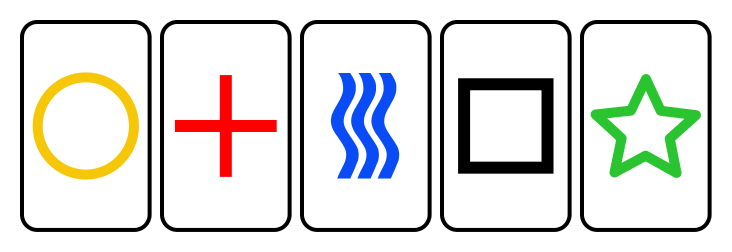
\includegraphics[scale=0.4]{zener.png}
	\caption{\href{https://commons.wikimedia.org/wiki/File:Zener_cards_(color).svg}{Zener Cards}, by Mikhail Ryazanov. Licensed under \href{https://creativecommons.org/licenses/by-sa/3.0/deed.en}{CC BY-SA 3.0}}
	\label{fig:zen}
\end{center}	
\end{figure*}



One often used experimental setup for testing ESP is an activity called
``card guessing'' using the so-called Zener cards, after Karl Zener, the
Duke psychologist who suggested the design to Rhine.\footnote{\cite{rhineesp},48} A Zener card can have one of 5
unique symbols. A typical deck of Zener cards contain 5 cards for each
symbol. A trial of this experiment typically involves a subject was
being repeatedly asked to guess the face of a randomly chosen card,
while the investigator would note the actual face of the card and the
subject's answer. After each trial, the subject's sequence would then
compared to the observed result, and a score would be calculated based
on the number of correct guesses.

Of course, one could achieve a high score by chance: no one would think
I had ESP if I successfully had predicted the outcome of a coin flip,
because we know that, no matter what my prediction is, I would still
have a \(0.5\) probability of getting it right. But what if I guessed 10
correctly the result of 10 consecutive tosses? The probability of that
is \(0.5^{10} = 0.001\). We are much more inclined to say that I have
some sort ability, because it would have been an extraordinary
coincidence if I got it right purely by chance. This is the sort of
statistical arguments that Rhine and his followers tried to make. Their
contention is that if a subject can obtain a score that is too
extraordinary to be explained by just chance, then we have statistical
evidence for the person's ESP ability. In statistics, the probability of
an outcome, assuming that it is by chance, is called the $p$ value.

Since there are 5 faces, a subject has the probability of \(0.2\) of
getting it right just by guessing alone, so someone with ESP should do
better than that. This is how ``better'' can be statistically
explicated: suppose a trial with 100 attempts has been carried out on a
subject. If the subject is just guessing, then we would expect that she
would get around 20 cards right. In fact, using the binomial
distribution, we can ascertain that out of 100 cards, there is a
probability of \(0.944\) that the subject can get 26 or less correct
guesses. Conversely, the probability that a guesser can get 27 or more
cards right is pretty low: the p value is \(0.056\).

Of course, this critical point entirely depends on how long the trial
is. In other words, we say that 27 is the cutoff, only because we
already decided that the trial involves 100 guesses. For 500 guesses,
for instance, there is a probability of 0.95 to randomly guess 115 cards
correctly. So, using the same standard, scores higher than 115 would be
considered as statistical evidence for the hypothesis the subject
actually has ESP.

\begin{table}[]
\centering
\begin{tabular}{l|c|c|c}
 Subject& Guesses &Hits  & Std. Dev. \\\hline
 M.C.& 1250 & 243 &  -0.49\\
H.F. &1000  & 219 & 1.50 \\
H.H. & 2000 & 416 & 0.90 \\
A.K. & 1000 & 212 & 1.50 \\
 H.S.& 1000 & 195 & -0.39 \\
 T.S. & 1000 & 222 & 1.73 \\
 J.T.& 1000 & 210 & 0.79 \\
 E.S.& 1750 & 370 & 1.19 \\
 A.M.& 500 & 118 & 2.01 \\
 L.S.& 500 & 113 & 1.45 \\
 D.A.& 750 & 168 &  1.64\\
 O.W.& 500 & 114 &  1.56
\end{tabular}
\caption{Summary of Performance Manic-Depressive Patients (Shulman, 1938, 101)}
\label{psychotable}
\end{table}

One study claims to have discovered just that: a parapsychologist
carried out the card guessing experiment on 141 patients in a mental
hospital.\footnote{\cite{psyesp}} The study claims to have found statistical evidence that
manic-depressive individuals have demonstrated the ability to detect the
face of a card through extrasensory means. It is said that these
subjects consistently scored higher than chance. For instance, consider
patient A. M. who got 118 hits out of 500 attempts. As discussed, it
would seem that, assuming A. M. was just guessing, it would have been an
extraordinary coincidence that he scored 18 higher than normally
expected. In fact, the p value---the probability for an outcome or
better like this to happen by chance---is \(0.027\), which is quite
improbable. Does this constitute evidence for ESP?

Feller argues that results such as this are spurious, because the
parapsychologists practiced \emph{optional stopping}. The idea is that
many of these experiments have no set number of attempts, and often
either an experiment could stop exactly when a favorable result is
obtained. For instance, an experiment could be terminated early in order
preserve a significant result. A. M., for instance, has made 500
attempts. His test was then much shorter than his peers, many of who
made more than 1000 guesses.

To make this point more concrete, we can take advantage of modern
statistical computing: we can simulate experiments with similar stopping
rules, and if we can get $p$ values below $0.05$. The difference here is that for the simulation we \emph{know}
that the participants are just guessing. So, if we can still force
significance using optional stopping, then there is a good reason to
doubt the supposed evidence for ESP. The scenario we need to simulate would be something like the following: the experimenter will randomly draw a Zener card out a shuffle deck, with replacement.
She will then ask the subject to guess the card, and record the result.
For each subject, she will stop under one of these two conditions: 1.
The result has reached significance: the probability of the current
outcome is less than \(0.05\). 2. 2000 guesses have been made. The
experimenter will then move on to the next subject, until she has
examined 1000 subjects. All subjects are guessing, so their probability
of success is exactly \(0.2\).

The simulation consists of the following procedure: \\


\begin{enumerate}
	\item The simulation will run 1000 times, each of which represents one subject. 
	\item For each subject $i$, a random sample will be drawn from a Bernoulli distribution, with the probability of success $p=0.2$, to simulate a subject who will randomly guess the face of a randomly drawn Zener card, with replacement. 
	\item For each draw $k$ for each subject $i$, the result $x_{i,j}\in \{0,1\}$ will be added to the total sum $y_i$ for the subject.
	\item Each trial run on indefinitely, \emph{until} one of the following conditions is obtained on the $n$th guess:\begin{description}
		\item[significance:] When the $p$ value is less than or equal to $0.05$. That is, 
		$$P(Y\geq y_i) = \sum_{j=y_1}^n {n \choose j} 0.2^j 0.8^{n-j}\leq 0.05$$
		\item[end:] $n=2000$: the subject has made 2000 guesses without significance. In this case, we simply move on to the next subject.
	\end{description} 
\end{enumerate}


Here's a summary of the result, after simulating testing 1000 subjects:

\begin{enumerate}
\def\labelenumi{\arabic{enumi}.}
\tightlist
\item
  371 out 1000 outcomes has reached significance. (\(p-value<0.05\)) In figure \ref{fig:freqhistp}, we see that the number of outcomes with significant p values far outnumbers the rest.
\item
  A p-value as low as \(0.017\) was obtained. A distribution of significant p-values can be see in figure \ref{fig:freqhistp}
\item
  On average, significant results stopped at the 294th attempt. The
  median is 85. According to figure  \ref{fig:freqhistn}, a substantial number of significant results were obtained by stopping before $400$ guesses. 
\item
  It would seem that successful tests tended to stop early, though this
  is not always the case. One test reached significant at the 1999th
  attempt.
\end{enumerate}

\begin{figure*}[h] 
\begin{center}
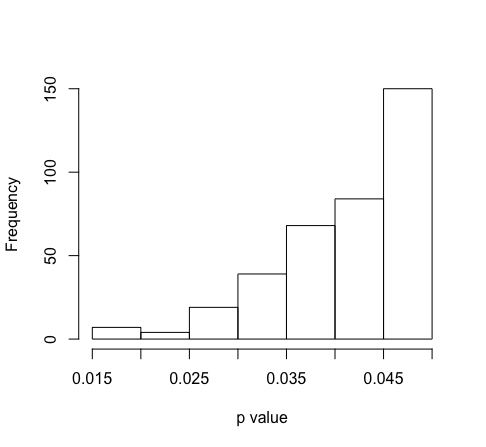
\includegraphics[scale=0.4]{freqstoppval.png}
	\caption{Histogram of p values $\leq 0.05$}
	\label{fig:freqhistpval}
\end{center}	
\end{figure*}

\begin{figure*}[h] 
\begin{center}
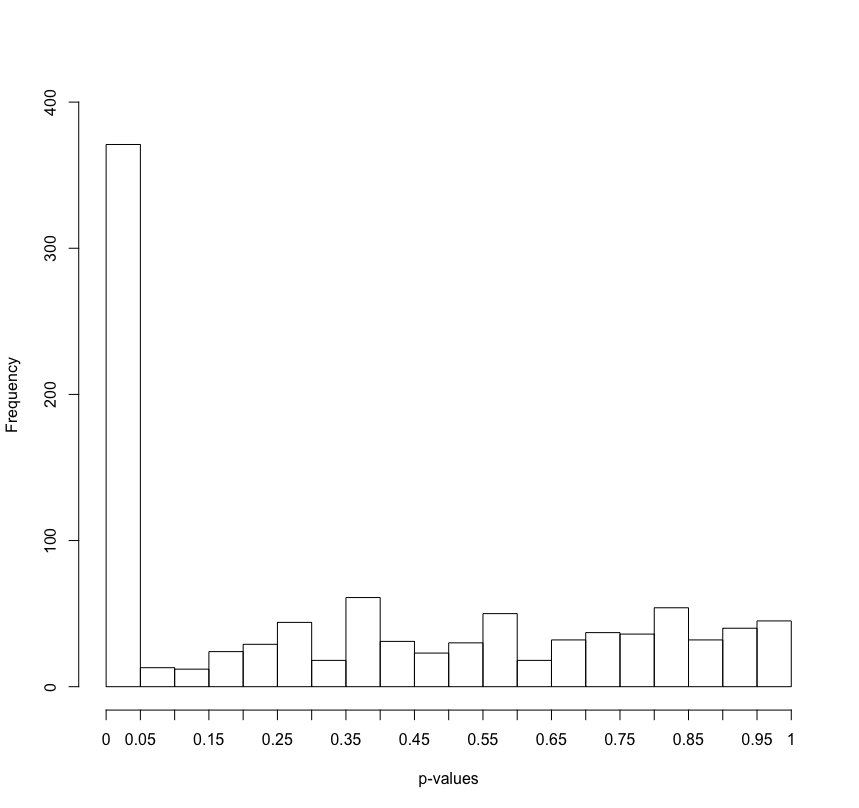
\includegraphics[scale=0.3]{freqstophist.png}
	\caption{Histogram of p-values from Optional Stopping Simulation}
	\label{fig:freqhistp}
\end{center}	
\end{figure*}

\begin{figure*}[h] 
\begin{center}
\includegraphics[scale=0.3]{freqstopn.png}
	\caption{Histogram of the Number of Trials Among Optionally Stopped Simulation}
	\label{fig:freqhistn}
\end{center}	
\end{figure*}


Thus, using optional stopping, we can easily find `evidence' for ESP if
we look long enough.

Even though Feller was primarily concerned with showing that many of the
findings in parapsychology is the result of shoddy experimental
practice, these problems would later be used by Bayesians as examples as
to why frequentism is flawed. The basic argument is that
parapsychologists could cheat in way they did, because of the way in
which the probabilities are computed and interpreted, and these problems
are supposed to avoidable within the framework of Bayesian statistics.
In the next section, we will review this argument.

\hypertarget{likelihood-and-counterfactual-probabilities}{%
\section{Likelihood and Counterfactual
Probabilities}\label{likelihood-and-counterfactual-probabilities}}

From the problem of optional stopping then, what follows? From the
Bayesian perspective, it suggests both a criticism of Frequentism and an
argument for Bayesian statistics. The criticism is that the
experimenter's intention to stop could directly influence the
significance of the result is because of frequentists' reliance of
\emph{counterfactual probabilities}. The defense is that Bayesian
methods do not require counterfactual probabilities, and therefore
immune to the argument from intention, and, therefore, is preferable. I
propose to first examine these two lines of thought, and then
transitions to the epistemological issues.

The implicit information here is that \(0.04\) is relative to what
\emph{would have} happened, if the the null hypothesis \emph{were} true.
To see what this means, note that there were 4 ways an experiment with
two attempts could have turned out. Let \(H\) to ``Hit'' and \(M\) be
``Miss''. The 4 possibilities are: \[MM \quad MH \quad HM \quad HH\] But
to get the probabilities needed, we will need to make at least one
additional assumption: we need to assume that the

because they are their respective probabilities are:
\[P(M\wedge M)=0.8^2=0.64 \quad P(M\wedge H)=0.2(0.8)=0.16\]
\[P(H \wedge M)=0.16 \quad P(H \wedge H)=0.04\]

The point Bayesians want to establish is that the p-values cannot be
seen as an unadulterated summaries of the observed evidence, since any
p-value is laden with assumptions about what might have happened, based
on some hypothesized parameters. In our comparison between the
likelihood function and sampling distribution, we have already touched
on the role of counterfactual probabilities in frequentist inferences.
According to many Bayesians, this is a one fundamental disagreement
between the two camps. Lindley says:


\begin{quote}
The usual statistical significance test requires the sample space, or alternatively, the stopping rule to be specified. Many people's intuition says this specification is irrelevant... Of what relevance are things that might have happened, but did not?\footnote{\cite{lindleybern}, 114.}
\end{quote}

Jaynes shares this sentiment:

\begin{quote}
The question of how often a given situation would arise is utterly
irrelevant to the question how we should reason when it does arise. I
don't know how many times this simple fact will have to be pointed out
before statisticians of ``frequentist'' persuasions will take note of
it.\footnote{\cite{jaynesmight},247}
\end{quote}

For many Bayesians, the problem of optional stopping is seen as a
decisive case against the frequentism and for Bayesianism. In
particular, Bayesians believe that the sort of problem caused by
optional stopping is due to the violation of the Likelihood
Principle(LP), which states, roughly, that everything one can learn from
an experiment about an hypothesis can be obtained by calculating the
probability of the \emph{actual} observation conditional on that
hypothesis. The reliance on \emph{only} actual observations, as opposed
to counterfactual ones, renders LP to be in a fundamental conflict with
frequentism. I. J. Good says the following that exemplifies this point
well:

\begin{quote}
Given the likelihood, the inferences that can be drawn from the
observations would, for example, be unaffected if the statistician
arbitrarily and falsely claimed that he had a train to catch, although
he really had decided to stop sampling because his favorite hypothesis
was ahead of the game. (This might cause you to distrust the
statistician, but if you believe his observations, this distrust would
be immaterial.) On the other hand, the ``Fisherian'' tail-area method
for significance testing violates the likelihood principle because the
statistician who is prepared to pretend he has a train to catch
(optional stopping of sampling) can reach arbitrarily high significance
levels, given enough time, even when the null hypothesis is true.\footnote{\cite{goodthinking},135}
\end{quote}

The use of the phrase `likelihood' here is technical: it refers to the
likelihood function \(p(x_{1:n}|\theta)\), which is the probability of
observations \(X_1...X_n\) conditional on the parameter of interest,
such as the probability of guessing a card correctly. The crucial point
here is that the likelihood function holds the actual observations to be
fixed, while the hypothesized parameter is variable. This is different
than the frequentist way, in which the \emph{hypothesis} is fixed, and
asks what the probabilities of different possible outcomes are, if the
hypothesis were true. This is why Bayesians repeatedly chide
frequentists for caring about data that we could have but didn't.
Likelihood function, the Bayesian way of summarizing data, does not take
into consideration of counterfactual probabilities at all.


\begin{table}[]
\centering
\begin{tabular}{@{}crrrr@{}}
\toprule
 & Factual & \multicolumn{3}{l}{} Counterfactual\\ 
Hypothesized Reliability & HH & HM      & MH      &  MM    \\\midrule
$0.2$ & 0.04 &   0.16    &   0.16    &    .64  \\
 $0.5$& 0.25 &    0.25   &   0.25    &    0.25  \\
 $1$& 1 &   0    &   0    &   0   \\ \bottomrule
\end{tabular}
  \label{tab:likelihoodvscf}
  \caption{Comparison between sampling distributions(rows) and likelihood functions(columns)}
\end{table}


At this point, the debate becomes quite messy, since Bayesians tend to
run the problem of optional stopping, and the likelihood principle
together, as Good has clearly done in the passage above. The assumption
is that optional stopping cannot occur once Bayesian methods are
adopted. However, the problem of optional stopping is perfectly
intelligible on frequentist ground: it draws out undesirable
consequences based on assumptions accepted by frequentists. The
introduction of LP, however, begs the question against the frequentists.
If all the fundamental frequentist methods violate LP, why would any
frequentist accept this principle? My suspicious is that they probably
won't.

However, what also motivates Bayesians to see LP as being indispensable
is that it allows statistical inferences to be made without caring
anything about the intentions of the experimenters. This attitude can be
summarized as \emph{the argument from intention}, which says that what
optional stopping shows is that Frequentist's reliance on counterfactual
probabilities renders their result vulnerable to manipulation, because
the experimenter's intention \emph{alone} can radically alter the import
of the evidence.

\hypertarget{intentions-and-self-sabotage-redux}{%
\section{Intentions and Self-Sabotage
Redux}\label{intentions-and-self-sabotage-redux}}

Consider a simple illustration concerning the bias of a coin discussed
by Lindley and Phillips.\footnote{D. V. Lindley and L. D. Phillips,
  ``Inference for a Bernoulli Process (a Bayesian View),'' \emph{The
  American Statistician} 30, no. 3 (1976): 113--14.} Suppose I was told
that the coin was tossed 12 times but out of those times 3 turned up
heads. The argument from intention says that, unless you know what goes
on inside the tosser mind when she decided to stop the tossing, there is
no way to know what the evidence says. And, depending on the answer she
gives, the evidential import of the result can alter drastically. For
instance, consider these stopping rules:

\begin{enumerate}
\def\labelenumi{\arabic{enumi}.}
\tightlist
\item
  Stop after 12 tosses
\item
  After 3 heads.
\end{enumerate}

The argument is that depending on which of the above rules the
parapsychologist used, the significance of the data will change, even if
the number of guesses and hits are the same. To begin, note that each
rule implies different impossibilities. For instance, if the
experimenter stops after 12 tosses, it is obviously impossible that the
test to last for more than 12 tosses, but it is possible for heads to
turn up as few as times and as many as 12 times. On the other hand, if
the test terminates after 3 heads, the only possible number of heads is
3, but the experiment can take as many tosses as needed to reach that
goal. So each different stopping rule implies different counterfactuals,
and leading to different sets of probabilities.

So Bayesians have an important point here: intentions are influencing
the statistical result through counterfactual probabilities, but, unless
there are reasons to think accounting for intentions is somehow
inherently bad, this \emph{supports} the deliberativist thesis, since
what it asserts is precisely that what agents intend to do to alter her
epistemic state is part of what deliberation is about, and therefore
must be considered in the interpretation of her data.

First, consider the rule that says stop after \(n=12\) tosses, so using
frequentist method means that we have to consider the probability of all
possible outcomes: that is, 0-12 heads. since a hit could occur at
different trials. We know that, from probability theory, for a random
variable with binary outcomes---success or failure, for instance---the
probability of getting \(k\) success out of \(n\) trials, given the
probability of a single success, is

\[{n \choose x} p^x (1-p)^{n-x}\]

Let's say a ``success'' is a coin toss that lands on heads. To carry out
an investigation, we have to make two decisions: the first is to choose
a hypothesis about \(p\) to be tested. In a binomial process with
\(n=12\), assuming that the coin's probability of landing on heads is
\(0.5\), what is the probability that she gets 3 or less heads? That is,
let \(Y=\sum_i^{12} X_i\), where \(X_i = 1\) if the coin lands on heads,
and 0 otherwise, then

\[P(Y \leq 3 ) =  \sum_{i=0}^{3} {12 \choose i} (0.5)^i (0.5)^{12-i} = 0.07\]

This is generally considered an insignificant result, but what if the
intention was to stop whenever the subject has gotten 3 heads? To model
this, we would have to use the so-called negative binomial distribution,
which models the probability making \(r\) failures before getting \(k\)
successes. In this case, the experimental question is in fact quite
different, since now we would consider the coin to be biased against
heads if it takes an abnormal large number of tosses possible. So the
statistical question is: what is the probability of the coin needing
\(12\) or more toss in order to get 3 heads? Using computers, we can
easily find this. Let \(X\) be the number of misses, so

\[P(X \geq 9) = 1 - P(X <9) = 1 - \sum_{i=0}^{8} {3+i-1 \choose i} (0.5)^3 (0.5)^{i} =0.03\]

This seems to be a much more significant result, but this is not the
complete picture. Given our discussion regarding abduction and
predesignation, the intention to stop's effect on statistical result in
fact strengthen the deliberativist position that inductive inference
must be understood against the background of an abductive context. The
stopping rule is one of those commitments that the agent needs to make
explicit prior the experiment, and changing it afterward is an act of
self-sabotage: it defeats the very purpose of trying to probe the
hypothesis accepted provisionally.

In the abductive context, it is true that there are decisions we are
free to make. There is no context-independent justification for the
choice of \(n\), which determine the probability of having \(k\)
successes. For instance, suppose we choose to toss the coin \(n=5\)
times, and that we decide on the hypothesis that \(p=0.5\). As Peirce
suggests, at this point I enjoy the voluntarist freedom of making any
epistemic judgment based on extra-evidential concerns: for instance, I
may only have time to throw the coin for 5 times. Just as breaking a
promise will cost my credibility, I have to specify how my obligation
can be resolved, in case my judgment turns out to be false. For
instance, a decision has to be made regarding how much deviation from my
own prediction is acceptable. This is where deduction takes over.

These decisions allow us to make deductions about the experimental
commitments that follow as necessary consequences from these parameters.
For instance, based on the model chosen, and that \(p=0.5\) and \(n=5\),
I can deduce that

\[P(X=0) = {5 \choose 0} 0.5^0 (1-0.5)^{5-0} = 0.031\]

\[P(X\leq 1) = \sum_{i=0}^1 {5 \choose i } 0.5^i (1-0.5)^{5-i} = 0.19\]

These are the probabilities that follow deductively from the decisions I
have been in the abductive context. I made what Peirce would call a
\emph{probable deduction}, which involves the deductive derivation of
probabilistic judgments based a model with known parameters. Even though
the conclusion of probable deduction is probabilistic, the
\emph{connection} between the conclusion and its premises is
necessary.\footnote{Peirce, ``A Theory of Probable Inference,'' 417.}
They signify the epistemic commitments I incur: if I accept
provisionally the hypothesis that \(p=0.5\) for \(n=5\), then I am
committed to the probabilistic judgment that the probability of tossing
the coin five times without heads is 0.031.\footnote{Of course, I could
  be dissatisfied by the result of the deduction, in which case I could
  revise my experimental commitment abductively. I put this issue aside
  now, as the dynamic between abduction and deduction is the focus on
  chapter 4.}

In any case, the point of the rule of predesignation is that once I have
made those decisions, \emph{I cannot revise them once I have started
flipping the coin}. I cannot, for instance, stop the experiment after
getting two tails in a row, only because I am interested in proving that
the coin is unfair. During abduction, I have made the commitment to stop
the experiment after 5 tosses---changing this intention changes the
whole inferential context altogether, and stopping early is an act of
self-sabotage. This can be shown by pointing out that the probability
getting two tails out of two throws is \(0.5^2 = 0.25\), which is much
higher than \(0.031\). We will discussion this problem with a greater
detail in the next chapter.

A crucial element in James' voluntarism is that the responsibility
implied by the inquirer's acceptance of a hypothesis includes the
incurring the risk of errors in rejecting the alternative hypotheses. To
get a grip on this risk, the agent must ask: what would happen, had I
accepted the wrong hypothesis? This style of thinking is already present
in Pascal's wager, in which he asks us to imagine the scenarios such as
mistakenly rejecting the existence of God or mistakenly accepting it.

This aspect of voluntarism is largely unaccounted for by the Reflection
Principle, but this Peircean framework I am describing can accommodate
by calculating so-called \emph{error probabilities}. For instance,
suppose I follow the standard practice and declare that I will reject
the hypothesis that \(p=0.5\), when the sample I collect has a less than
the probability of \(0.05\) of occurrence. This would mean that I am
committed into rejecting my hypothesis if I get no heads after tossing
the coin 5 times. But what if the coin is actually biased, but not
insofar as it would not even once land on heads? The probability of
making such an error can be calculated \emph{ex ante} deductively. For
instance, suppose the reality is that the coin is biased such that
\(p=0.2\). But if this were true, I have a high probability of keeping
my provisionally accepted hypothesis by mistake, because

\[P(X > 0) = 1 - P(X=0) = 1 - {5 \choose 0} 0.8^5 = 0.67\]

This means that by accepting \(p=0.5\), I am incurring a pretty high
risk of error: if \(p=0.2\), there is a 0.67 probability that I will
come to error. The closer \(p\) is to \(0.5\), the more likely it is
that I will come to accept \(p=0.5\) erroneously. If \(p=0.3\), for
instance, this error probability is \(0.83\). Of course, incurring the
risk of error matters only if I care about finding out the truth. If all
I care about is to confirm my hypothesis, incurring the high risk of
error will not be counted as genuinely accepting an obligation---it
would be similar to promising to eat lunch today, which I would do
regardless of the promise anyway. This is why Peirce insists that
validity of inductive inference depends on

\begin{quote}
first, a sense that we do not know something, second, a desire to know
it, and third, an effort,---implying a willingness to labor,---for the
sake of seeing how the truth may really be.\footnote{Peirce, \emph{The
  Essential Peirce, Volume 2}, 1998, 48.}
\end{quote}

Thus, we can understand the problem of optional stopping as a special
case of \emph{self-sabotage}: that is to preemptively sabotaging one's
possibility of ``seeing how the truth may really be''. Of course, this
is a self-sabotage only if the agent cares about the truth at all.

Returning to Lindley's case of getting 3 heads of 12 tosses. He is
entirely correct in pointing out that under different stopping rules
would have an impact on what will counted as statistical significance,
even if the numerical result will be the same, but from the
deliberativist standpoint, these stopping rules imply different sets of
epistemic commitments.

If the agent intends to stop after 12 trials, then to aim for a level of
statistical significance \(\alpha\) at \(0.05\), she would have to
commit to reject the fair coin hypothesis if she gets 2 or less heads.
The repercussion is that, had the coin been only slightly biased against
landing on heads, it is unlikely that she would be able to find the
truth. For instance, the probability getting 2 or less heads, if
\(p=0.4\), is only \(0.08\). For \(p=0.3\), it's \(0.25\). In other
words, if the coin were only slightly biased, it would unlikely to
produce the result that is detectable within this particular
deliberative framework. Of course, there is nothing sacred about
\(\alpha= 0.05\), notwithstanding the preaching of introductory
statistics textbooks. If the agent's intention is to determine if the
coin is only slightly biased, she is free to adjust \(\alpha\) so that
her risk of error, had \(p\) been \(0.4\), is smaller. Even though, if
\(p=0.5\), the probability of getting 3 or less heads out of 12 at
\(0.07\) does not quite reach the textbook standard of statistical
significance, it nevertheless would be much better at detecting
\(p=0.4\), since the probability of the same outcome occurring would be
\(0.23\). Not perfect, but this is the kind of decision one makes during
the abductive context.

None of the above considerations hold if we had changed the stopping
rule to ``stop after 3 heads.'' The deliberative framework would be
entirely different. To begin, we are now adjudicating, not the
probabilities of error between different numbers of heads landed, but
the number of tails we would tolerate before 3 heads is seen. We saw
that having to see 9 tails before 3 heads is a statistically significant
enough reason to reject the hypothesis that the coin is fair. What this
overlooks, however, is that a biased coin can often get 3 heads before 9
tails; because, probabilities from a negative binomial distribution tend
to be ``front-loaded''. For instance, with a coin that is half as
unlikely to land on heads than tails, that is, \(p=0.25\), the
probability to see 8 or less tails before 3 heads is

\[P(X \leq 8) =  \sum_{i=0}^{8} {3+i-1 \choose i} (0.25)^3 (0.75)^{i} =0.55\]

So looking strictly at the different p-values is a somewhat misleading
way to look at the matter. Mayo and Spanos summarizes the frequentist
response as follows:

\begin{quote}
{[}the argument from intention{]} would seem to beg the question against
the error statistical {[}i.e., frequentist{]} methodology which has
perfectly objective ways to pick up on the effect of stopping rules: far
from intentions ``locked up in the scientist's head'' (as critics
allege), the manner of generating the data alter error
probabilities\ldots{}\footnote{Deborah G. Mayo and Aris Spanos, ``Error
  Statistics,'' in \emph{Handbook of the Philosophy of Science, Vol. 7:
  Philosophy of Statistics}, ed. Prasanta S. Bandyopadhyay and Malcolm
  R. Forster (Elsevier B.V., 2011), 186.}
\end{quote}

Of course, a defense of intentions in frequentism is not an argument
\emph{for} the relevance of intention in Bayesianism. Furthermore,
Bayesians like Lindley without a doubt was aware of these basic
statistical facts from power analysis. What prompted their stance is the
assumption that Bayesian methods are impervious to the problem of
optional stopping, since the likelihood function is not affected by
intentions, or other facts in the deliberative framework. In the next
section, I will demonstrate that optional stopping can also affect
results obtained using Bayesian methods, so I am attacking the very idea
that Bayesians cannot ignore the effects of deliberation.

\hypertarget{bayesian-early-stopping}{%
\section{Bayesian Early
Stopping}\label{bayesian-early-stopping}}

Deborah Mayo suggests that using early stopping to manipulate experimental result is also possible using Bayesian method, despite of the Likelihood Principle.\footnote{\cite{errorgrowth},352-353} Mayo's argument appeals to the fact that Bayesian methods can obtain the same or similar result when using a flat/uninformed prior, so this opens the door to early stopping using the same method. I will try to get more mileage out of this argument by using simulations.

To begin, we have to gain an understanding of what Bayesian inference is
like. Naturally, it begins with Bayes' theorem. Consider some hypothesis
or belief \(H\) and some evidence \(E\).

\[P(H|E) = \frac{P(H)P(E|H)}{P(E)}\]

In its most basic form, Bayes' theorem has 3 components: The
unconditional probability of \(H\), \(P(H)\) represents the probability
we would assign to the belief before the evidence, which, as we have
discussed, is represent by the likelihood \(P(E|H)\)---the probability
of the evidence, given the hypothesis is true. The third ingredient is
\(P(E)\), the unconditional probability of \(E\). To see how this works,
consider an example with Zener cards. To begin, suppose that we have a
subject in front of us, and we have to determine she has ESP. Let's say
she has 2 out of 2 correct answers. How should we learn from this data?
What follows is the standard Bayesian story.

For the sake of simplicity, for now let us suppose that there are only
two options: either the subject is randomly guessing, or she has ESP,
which entails a perfect reliability. In other words, we have two
hypotheses. Let \(\theta\) be the subject of probability of getting a
hit, and

\begin{enumerate}
\def\labelenumi{\arabic{enumi}.}
\tightlist
\item
  \(H_0: \theta = 0.2\)
\item
  \(H_1: \theta = 1\)
\end{enumerate}

These are sometimes called ``chance hypotheses.'' Now let \(E_i\) refers
to the result of the \(i\)th guess, and it equals \(1\) for a hit, and
\(0\) otherwise. So let \(E = \sum_i^2 E_i = E_1 + E_2 = 2\). This means
that we have the following likelihoods:

\begin{enumerate}
\def\labelenumi{\arabic{enumi}.}
\setcounter{enumi}{2}
\tightlist
\item
  \(P(E|H_0) = 0.2^2=0.04\)
\item
  \(P(E|H_1) = 1\)
\end{enumerate}

Recall that the likelihood principle says that this contains all the
information we need to know about the experiment. Now, suppose you are
not a believer of ESP, so you are almost certain---say, \(99\%\)
sure---that the subject will not do better than chance. We then have the
priors needed:

\begin{enumerate}
\def\labelenumi{\arabic{enumi}.}
\setcounter{enumi}{4}
\tightlist
\item
  \(P(H_0) = 0.99\)
\item
  \(P(H_1) = 0.01\)
\end{enumerate}

From the above, we can derive
\[P(E_i = 1) = P(H_0)P(E_i=1|H_0) + P(H_1)P(E_i=1|H_1) = 0.99(0.04)+0.01(1) = 0.0496\]

Using Bayes' theorem, we can then revise our belief about the subject's
ability to guess cards, producing the following \emph{posterior
probabilities}:

\[P(H_0|E) = \frac{0.99(0.04)}{0.0496} = 0.8\]
\[P(H_1|E) = \frac{0.01(1)}{0.0496} = 0.2\]

Having seen two successful attempts in a row, we have warmed up to the
idea that the subject might have ESP. An intuitive way to look at this
Bayesian procedure is that the posterior probability is a promise
between my existing belief---my priors---and evidence, which is
summarized by the likelihoods, according to the LP.

To make my point, these basic Bayesian statistical procedures are
sufficient, though things will get somewhat messy when we consider more
realistic cases. For instance, it is arbitrary to consider only two
chance hypotheses. A more applicable model would be to consider all
possible values of \(\theta\) in \([0,1]\). For that we have to use some
of the well-established distributions. I will use again use simulation
to demonstrate the effect of optional stopping, but to do so I need to first explain
how the situation will be modeled.

Recall that optional stopping from a frequentist context entails
falsely rejecting null hypothesis by sampling over and over again until
obtaining an outcome with a probability low enough on the null
hypothesis to secure statistical significance. The Bayesian parallel is
to keep on sampling so we can have \(E\) such that \(P(H_0|E) < x\)
where \(x\) is a value the optional stopper is committed into believing.
Note that now we are talking about the probability of the hypothesis
itself, whereas in the frequentist setting we were concerned with the
probability of the observation.

Fortunately, since there are only two outcomes, a Zener card-type
experiment can be modeled as a Beta-Bernoulli process, where the Beta
distribution would model our degrees of belief about a subject's
\emph{propensity} and the Bernoulli distribution would represent the
Zener card experiment itself. What these models represent is usually
clear enough in a practical and statistical setting, but since we are doing philosophy, we need to be clearer about what we mean by
degrees of belief and propensity, so we are clear about the phenomena being
modeled.

I suggest we follow the views of D. V. Lindley and David Lewis. Lindley
argues that probability is a relation between the agent and the world,
so when we say \(P(\theta=0.5)\), it represents our epistemic judgment about some physical event \(\theta\).\footnote{\cite{lindleybern}, 115.} In our case, this
has to be an objective reliability of the subject's ability to discern the face of the card, which
is a property in the world: even though \(\theta\) looks like a
probability, in the Bayesian statistical framework we can just treat it
as another parameter being modeled, not unlike \(\mu\) or \(\sigma\) for
normal distributions, so a subject's extra-perceptual reliability is a
objective feature of the world in a way no different than the fact that
the average age of Duke students is an objective fact. The degree of
beliefs about them, according to the voluntarist conception I accept, is an epistemic judgment made about this objective fact.
 
 This recommendation is compatible with, if not the same as, the influential
view presented by David Lewis, who adopts Carnap's pluralistic stance on
probability. Carnap thinks there are at least two concepts of
probability: \(probability_1\), which is an epistemic concept about
degrees of confirmation and \(probability_2\), which refers the
empirical concept of long-run limiting frequencies.\footnote{\cite{carnapprob}, 517.} Lewis suggests
that we should instead interpret the epistemic concept as credence or
degree of belief and the empirical concept as chance or
propensity.\footnote{\cite{lewisguide}} So, following Lewis, we can interpret \(P(\theta=0.5)=x\) to
be ``the degree for the belief that the chance of heads is 0.5 is
\(x\).'' For the sake of consistency, I will refer to subjective
probability just as \emph{credence} or \emph{degrees of belief}, and
objective probability as \emph{chance} or \emph{propensity}.

We can now spell out the type of experiments that will be simulated.

Early on, we considered a case in which only two possible hypotheses are
considered: either the subject is guessing
randomly(\(H_0:\theta = 0.2\)) or the subject has perfect
reliability(\(H_1:\theta = 1\)). This makes our epistemic attitude
relatively easy to summarize, since all we have to do is to assign a
value to our credence to each of the two hypotheses. As we noted, this
is an oversimplification, since there is no reason to arbitrarily
restrict ourselves to just two hypotheses. This, however, means that we
need a way to deal with the fact that there are infinitely many possible
hypotheses between 0 and 1, which is why we need the beta distribution.

The beta distribution is really nothing but a function that, based on
two parameters we provide, describes our epistemic attitudes toward
\(\theta\).\footnote{The distribution has the form:
  \(\frac{\Gamma(\alpha + \beta)}{\Gamma(\alpha)\Gamma(\beta)}x^{\alpha -1} (1-x)^{\beta -1}\)
  where the parameters \(\alpha,\beta > 0\) and
  \(0\leq x \leq 1\)(\(x\) is the random variable being
  modeled) } The two parameters, \(\alpha>0\) and \(\beta>0\), can be
thought of as, in our context, our past experience about \(\theta\),
with \(\alpha\) representing past successes and \(\beta\) past failures.
For instance, if we set \(\alpha = \beta = 1\), it should say that we
are extremely ambivalent about \(\theta\). In fact, it is equivalent to
having a uniform distribution over \([0,1]\)---this means that I am
utterly indifference regarding any value for \(\theta\).

Our data-collection will be modeled using the binomial distribution. Let
\(x\) be the number of success, \(n\) the number of trials, and
\(\theta\) the propensity of success:

\[f(x|\theta, n) = {n\choose k} \theta^k (1-\theta)^{(n-k)}\]

This is the same distribution we used as the sampling distribution in
the frequentist case, but recall that for Bayesian analysis we will no
longer concern ourselves with counterfactual probabilities, instead, we
are treating \(\theta\) as the function of the \(x\), the number of
success which is constant.

Fortunately, as soon as this is laid out, the rest is very simple,
thanks to the fact that the beta distribution is a \emph{conjugate
prior} for the binomial distribution. Essentially, what this mean is
just that if we plug the beta and binomial distributions into Bayes'
theorem to get a posterior distribution

\[ p(\theta|x) = \frac{p(\theta)p(x|\theta)}{\int p(\theta)p(x|\theta)}\]

\noindent the result is simply another beta distribution with parameters
\(\alpha =\alpha + x\) and \(\beta = \beta + n - x\). In words, to learn
from experience, all we have to do is to add the number of successes to
\(\alpha\) and the number of failures to \(\beta\). Another useful thing
to keep in mind is that the beta distribution's expected value has the
form:

\[E(\theta) = \frac{\alpha}{\alpha + \beta}\]

\noindent Now, because of a very nice property called conjugacy, the \emph{posterior} expected value
is simply:

\[E(\theta) = \frac{\alpha + k}{\alpha + \beta + n}\]

So, our experimental procedure is fairly simple: we pick an appropriate
set of parameters, and for each trial in which the subject is able to
guess the card correctly, we add 1 to \(\alpha\); otherwise, we add 1 to
\(\beta\). For example, consider again the case of a skeptic who
observed that a subject has made two correct guesses in a row. Since
prior the observation the skeptic does not believe that the subject
would do better than chance, she knows that

\[E(\theta) = \frac{\alpha}{\alpha + \beta} = \frac{1}{5}\]

There are various ways in which we can make this work mathematically,
but for now let's say \(\alpha = 2\) and \(\beta = 8\). \footnote{The epistemological relevance of the choice of these parameters will the discussed in chapter \ref{ch:woe}.} Since the
subject has gotten 2 out of 2 correctly, the skeptic's posterior should
be the beta distribution with \(\alpha= 2+2=4\), while \(\beta\) remains
at 8.

Because we are using Bayesian methods, we can ask directly the
probability of \(\theta\) having certain values. A similar question we
can ask, then, \emph{given} the evidence we have, what is the
probability of the subject's para-perceptual reliability is no better
than randomly guessing? In other words, what is the probability that
\(\theta\) is less than or equal to \(0.2\)? Using the cumulative
distribution function for the beta distribution using standard
statistical software, we can find out the prior and posterior values:

\[P(\theta \leq 0.2) = 0.56\] \[P(\theta \leq 0.2|\mathbf{X}) = 0.16\]

We can see that after witnessing the evidence, the skeptic's personal
probability for the belief that the subject is doing no better than
chance is lowered by quite a bit. The Bayesian version of optional
stopping is this: a Bayesian optional stopper can decide to stop
gathering more evidence as soon as the posterior is low enough. The idea
is that a committed enough optional stopper will eventually find
``evidence'' for ESP, i.e., subjects with low posterior probability of
random guessing.

To simulate this procedure, we will carry out the following:



\begin{enumerate}
\def\labelenumi{\arabic{enumi}.}
\tightlist
\item
  Loop for \(n\) times for \(n\) subjects.

  \begin{enumerate}
  \def\labelenumii{\alph{enumii}.}
  \tightlist
  \item
    For each subject \(s\), we begin with a flat uniform distribution by
    setting \(\alpha = \beta = 1\).
  \item
    A random sample \(x_i\) will be drawn from a Bernoulli distribution,
    with \(\theta = 0.2\).
  \item
    Add 1 to \(\alpha\) if \(x_i =1\); add 1 to \(\beta\) otherwise.
  \item
    Terminate if either (i) \(P(\theta_s \leq 0.2|\mathbf{X})\) is less
    than threshold \(k\leq 0.05\) or (ii) the number of trial \(i\) has exceeded
    the maximum number \(m=2000\). Otherwise, return to step a with the same
    subject.
  \end{enumerate}
\item
  If \(n\) subjects have been tested, terminate; else, return to step a
  with a new subject.

\end{enumerate}



\begin{figure*}[h] 
\begin{center}
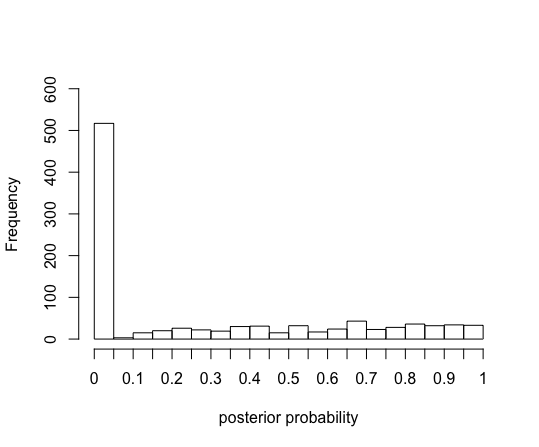
\includegraphics[scale=0.5]{Bayesstopflatallpost.png}
	\caption{Histogram of $p_i(\theta\leq 0.2|x,\alpha=1, \beta=1)$}
	\label{fig:bayesflatposterior}
\end{center}	
\end{figure*}

\begin{figure*}[h] 
\begin{center}
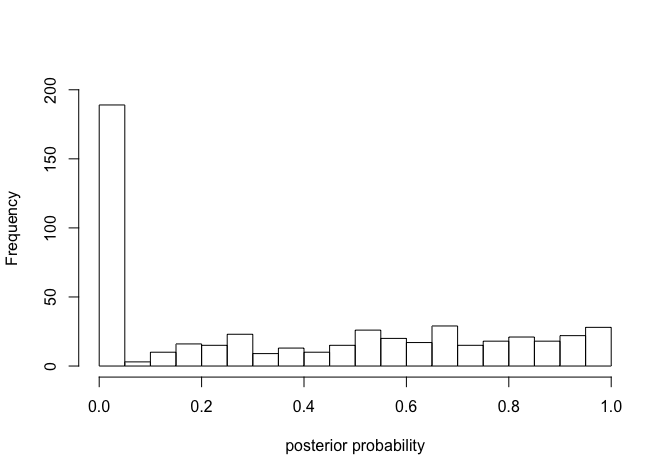
\includegraphics[scale=0.5]{bayesstop14allpost.png}
	\caption{Histogram of random samples from $p_i(\theta\leq 0.2|x,\alpha=1, \beta=4)$}
	\label{fig:bayes14posterior}
\end{center}	
\end{figure*}

$n=1000$ stimulations were carried out. We clearly see the effect of early stopping here. In fact, using a flat prior, $\alpha=\beta=1$, 517 out of 1000 stimulations were stopped early due to reaching a low enough posterior probability for $p(\theta \leq 0.2)$, which more than the number we had for frequentist early stopping. The distribution of the posterior probabilities can be seen in figure \ref{fig:bayesflatposterior}. This is partly due to the fact that, when starting from a flat prior, the  experiment can stop after 1 guess if the first guess is the correct one, because with $\alpha = 2, beta=1$, the posterior probability for $P(\theta\leq 0.2 = 0.04$, which is already lower than the threshold designated. 208 out of 1000 simulations ended this way, which is exactly what was expected, since we are drawing from a Bernoulli distribution with the probability $0.2$ of success. 

To eliminate that particular result, we can use a weakly informed prior, by setting $\alpha = 1, beta=4$. The result is summarized in figure \ref{fig:bayes14posterior}. Since the initial expected value is $0.2$, and this means that for the cases in which early stopping is successful, we have essentially manipulated ourselves from the right opinion into the wrong one. The result is nearly identically to the frequentist case, with 367 out of 1000 results being stopped early to get the posterior probability desired.


Based on the above, one may argue that optional stopping could further prevented by using a even strongly informed prior. This is true: for instance, if, instead of
having \(\alpha = \beta = 1\) as parameters, we use something strongly
biased in favor of \(\theta = 0.2\), such as
\(\alpha = 10, \beta = 40\), it would be fairly difficult for the
optional stopper to game the result. But this makes sense only because we \emph{know} what the true distribution is. This also seems to me a point
\emph{for} deliberativism, not against it, because this is amount to
saying commitments and intentions matter by sneaking them in through the
back door of priors. Furthermore, what is stopping an optional stopper
to cheat even more by adopting a set of parameters that is biased
\emph{against} \(\theta = 0.2\)? Of course, we would criticize anyone
that adopts such an experimental stance, but it would be made on the
deliberativist ground.

\hypertarget{is-optional-stopping-irrational-from-the-perspective-of-the-utility-maximizer}{%
\section{Is Optional Stopping Irrational From the Perspective of the
Utility
Maximizer?}\label{is-optional-stopping-irrational-from-the-perspective-of-the-utility-maximizer}}

There is, however, a more substantive objection that requires a more
thorough exposition. An Orthodox Bayesian could argue that optional
stopping is an irrational practice, because from a Bayesian perspective
it is never rational to refuse evidence, because additional evidence
\emph{always leads the increase in expected utility}. This is in fact a
result that has been proven in various occasions and forms by Frank
Ramsey, I. J. Good, and L. J. Savage.,\footnote{F. P. Ramsey, ``Weight
  or the Value of Knowledge,'' \emph{British Journal for the Philosophy
  of Science} 41, no. 1 (1990): 1--4.}\footnote{I. J. Good, ``On the
  Principle of Total Evidence,'' \emph{British Journal for the
  Philosophy of Science} 17, no. 4 (1966): 319--21.}\footnote{Savage,
  \emph{The Foundations of Statistics}, sec 6.2.}

Some context is helpful. In his \emph{A Treatise in Probability}, J. M.
Keynes points out that subjectivists and expected utility theorists
often implicitly assume that we should always get more evidence.
Bernoulli, for instance, suggests that rationality demands the
utilization of all evidence available to us. This implies, Keynes
thinks, that it's always rational to get more evidence, but then it
raises another critical question about whether or not one could ever be
rational in refusing new evidence.\footnote{Keynes, \emph{A Treatise on
  Probability}, 84--85.} If the answer for the former question is
positive, and the latter question negative, then we have to conclude
that rationality dictates us that we should never stop looking for more
evidence. This problem received little attention, except by Ramsey in an
unpublished note, until years later Ayer raises the same question in
response to Carnap's \emph{Logical Foundation of Probability}, in which
Carnap essentially restates Bernoulli's maxim as ``the requirement of
total evidence''.

\begin{quote}
\emph{Requirement of total evidence}: in the application of inductive
logic to a given knowledge situation, the total evidence available must
be taken as basis for determining the degree of confirmation.\footnote{Carnap,
  \emph{Logical Foundations of Probability}, 211.}
\end{quote}

Ayer asks the Keynesian question: should ``total evidence'' include
relevant evidence that I do not yet have in possession?\footnote{A. J.
  Ayer, \emph{Probability and Evidence} (Macmillan, 1972), 56.} The
answer must be ``yes'', Ayer argues. If finding the truth value of some
proposition \(P\) could potentially sway the balance of my evidence,
then I should definitely acquire it. Thus the principle of total
evidence seems to suggest that I am also rationally compelled to
consider some evidence I do not yet have.

I. J. Good interprets Ayer's as questioning ``why\ldots{} we should
bother to make new observations.''\footnote{Irving J. Good, \emph{Good
  Thinking: The Foundations of Probability and Its Applications} (Univ
  Minnesota Pr, 1983), 178.} In the context of optional stopping, this
is particularly salient: if I already have the result I want, why should
I bother get more evidence?

Ramsey, in an unpublished note, was the first one to address this
problem from a Bayesian perspective. Ramsey's argument is roughly that,
\emph{if} we assume an agent to be a perfect Bayesian and that new
information does not cost anything, then she will never be no worse off
getting new evidence. In fact, she is guaranteed to be \emph{better} off
as long as the new evidence will tell her something new. A perfect
Bayesian agent is someone who studiously updates her opinions based on
Bayes' rule and then act by choosing the action that maximize her
expected utility. Note that this assumes two things: first, for any
decision problem she faces, there is always going at least one course of
action that maximizes her expected utility, and second, as Skyrms points
out, this also implies that the agent knows that she will always
\emph{stays} being perfectly Bayesian in the future. What we have here,
then, is the ideal Bayesian agent.

I will make use of an intuitive example rather than reproducing the
proof here.\footnote{This example is adapted from Isaac Levi, ``The
  Weight of Argument,'' in \emph{Fundamental Uncertainty: Rationality
  and Plausible Reasoning}, ed. Silva Marzetti Dall'Aste Brandolini and
  Roberto Sczzieri (Palgrave MacMilan, 2011), 39--58} Suppose we have
three hypotheses about the content of an urn in front of us:

\begin{enumerate}
\def\labelenumi{\arabic{enumi}.}
\tightlist
\item
  \(H_b\): 90 black balls and 10 white balls
\item
  \(H_w\): 10 white balls and 90 black balls
\item
  \(H_n\): 50 white balls and 50 black balls.
\end{enumerate}

Suppose we start by assuming \(P(H_b) = P(H_w) = P(H_n) = 1/3\)---we
could have some knowledge that assures us that these are the only three
possibilities. There is also a reward of \$1 for picking the correct
hypothesis. Our expected payoff for choosing each hypothesis would be
the same at \(1/3\). Nevertheless, we are allowed to sample with
replacement as many times as we wish. Should we get more evidence? Yes,
according to Ramsey, we should, and this can demonstrated in terms of an
expected utility analysis.

To begin, at this point, the probability of getting a black ball is the
same as getting a white ball. Let \(E_b\) be ``a black ball is drawn''
and \(E_w\) for white balls. So:
\[P(E_b) = P(H_b)P(E_b|H_b) + P(H_w)P(E_b|H_w) + P(H_n)P(E_b|H_n)\]
\[=1/3(0.9)+1/3(0.1)+1/3(0.5)=0.5\] And \(P(E_w) = 1 - P(E_b) = 0.5\).
So, in the event of drawing a black ball from the urn, we would update
our belief like so:

\[P(H_b|E_b) = \frac{P(H_b)P(E_b|H_b)}{P(E_b)}=\frac{1/3(0.9)}{0.5} = 0.6 \]

Similarly, applying the calculation on the other hypotheses, we get:
\[P(H_w|E_b) = 0.067\] \[P(H_n|E_b) = 0.333\] Similar argument can be
made by assuming \(E_w\), that is, a white ball is chosen. In that case
\(P(H_w|E_w) = 0.6\). If we were an ideal Bayesian agent, we should pick
\(H_b\) if \(E_b\), and pick \(H_w\) if \(E_w\). Since an ideal Bayesian
would choose the option that maximizes our expected utility, in either
case the expected value after drawing from the urn once is \(0.6\),
which is an improvement, since before drawing our expected utility is
\(1/3\) for all options. The net gain in expected utility would be
\(0.6 - 0.33 = 0.27\), is referred to as \emph{the value of information}
in the decision theory literature.\footnote{Howard Raiffa and Robert
  Schlaifer, \emph{Applied Statistical Decision Theory} (Harvard, 1964),
  89--90. For a more digestible presentation see @winkler sec.6.3.}

It turns out that we would be even better off if we were to draw from
the urn again. Suppose the first draw yields a black ball. So now we
have one piece of evidence in hand. Let us refer to our state of belief
after the first draw as \(H_b', E_b',..\) and so on. For instance,
\(P(H_b') = P(H_b|E_b)\) and \(P(E_b') = P(E_b'|E_b)\). One notable
change is that \(P(E_b') = 0.7132\) and \(P(E_w')=0.2868\). If we draw
again and get a black ball, this means:

\[P(H_b'|E_b') = 0.757\] \[P(H_w'|E_b') = 0.009\]
\[P(H_n'|E_b') = 0.233\]

If a white ball were to be drawn:

\[P(H_b'|E_w') = 0.21\] \[P(H_w'|E_w') = 0.21\] \[P(H_n'|E_w') = 0.58\]

Thus, if the second sample is a black ball, we would choose \(b\) since
it has the maximum expected utility at \(0.757\), and if we get a white
ball, we choose \(n\) with the expected value at \(0.58\). So, the
expected utility, if we were to draw from the urn again, is:
\(0.7132(0.757) + 0.2867(0.58) = 0.706\), which is an improvement over
just drawing once. The net gain is \(0.706 - 0.6 = 0.106\). Ramsey's
proof shows that we can keep on getting more evidence and we will never
be worse off. In fact, we will be better off as long as there is
evidence out there we do not yet have.

To see a bird's-eye view of the situation, consider figure \ref{fig:expectedchange}, in which the sequential updatings of expectation after drawing from different hypothesized distribution are plotted. Each line represent the \emph{net change} of expected value of getting more evidence conditional having $x$ observation. We can see that the expected net change will never dip below $0$, meaning that one will always often be rewarded and never punished for getting more evidence.

\begin{figure*}[h] 
\begin{center}
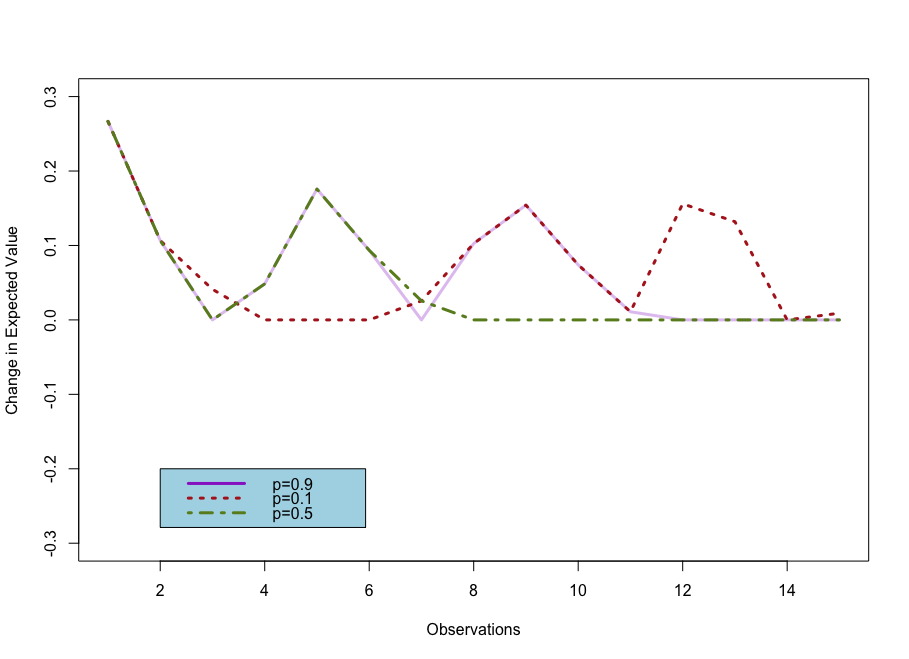
\includegraphics[scale=0.5]{Expectedchange.png}
	\caption{Net change in expectation after $x$ observations from $p=0.9,0.1,0.5$. Note: it does not dip below 0.}
	\label{fig:expectedchange}
\end{center}	
\end{figure*}


This result could be used to answer the Bayesian version of optional
stopping in this way: since getting more evidence always yields better
expected values, the ideal Bayesian agent will always opt for more
evidence, instead of stopping ahead just because the posterior has
reached her favorite degree.

However, I do not think this answer will do. To begin, the crucial
assumption here is that evidence costs \emph{nothing}. The scenario we
imagined quickly breaks down once we starts to introduce some sort of
cost. It was assumed in the example that it costs us neither money nor
time to draw from the urn, but suppose it costs us 25 cents for each
sample. This means that we would be gaining only \(0.27-0.25 = 0.02\) in
expected payoff for the first draw, and the second draw would definitely
not be worth the additional 25 cents. Or suppose that one dollar is not
worthy any endeavor that lasts longer than 15 seconds, and it takes 30
seconds to draw from the urn. As soon as minimally realistic assumptions
are introduced, Ramsey's result no longer holds.

Cost might also enter into consideration in different forms. Savage
ponders over a case in which a very ill person, who is given the option
to find out with no financial cost if the disease she has is terminal.
Savage points out that an argument can be made that in this case
refusing information could be rational. The thought is that the patient
may decide that, based on an assessment of her own personality, she
would live the rest of her remaining life in agony if she were to find
out that her disease is very serious, whereas she could live relatively
happily without knowing. Savage's point is that in this case the
information is not really free; it has a \emph{psychological}
cost.\footnote{Savage, \emph{The Foundations of Statistics}, 107.}

Ramsey and Good's proofs, while extremely valuable from a logical and
mathematical perspective, are somewhat tone-deaf to the actual problem
posed by Ayer and Keynes. The actual complaint was that the Principle of
Total Evidence \emph{presupposes} that we know ahead what ``total
evidence'' amounts to, since the decision to get more evidence or simply
sticking to our current body of evidence is not one that be resolved
just by appealing to probability, because the rationality of such a
decision is highly context-sensitive. One important context is the
\emph{urgency} of decision. For instance, ``a general who refused to
launch an attack until he had ascertained the position of every enemy
solider would not be very successful.''\footnote{Ayer, \emph{Probability
  and Evidence}, 57.}

The economist G. L. S. Shackle makes a similar point engagingly by
retelling the thought process of a certain Chinese guard who had to
decide on the spot whether or not to join the rest of the guards to
partake in a rebellion or to be the lone loyalist to stand in defense of
the empire. He argues that it would be rather foolish to suggest that
the guard should maximize his utility by looking for more evidence:

\begin{quote}
{[}Had the guard taken heed of the advice given by the expected utility
theorist,{]} he might have argued thus: `I find in the record of history
a thousand cases similar to my own, wherein the person concerned decided
upon treachery, and in only four hundred of these case the rebellion
failed to and he was beheaded. On balance, therefore, the advantage
seems to lie with treachery, provided one does it often enough'\ldots{}
Had the sentry decided to support the rebellion, he might have had time,
just before the axe fell, to reflect that he would never, in fact, be
able to repeat his experiment a thousand times, and thus the guidance
given him by actuarial considerations had proven illusory.\footnote{G.L.S.
  Shackles, \emph{Uncertainty in Economics and Other Reflections}
  (Cambridge University Press, 1955), 2.}
\end{quote}

My point, of course, is not that making decision based on probability
and utility is irrational. Far from it, but, again, that rational
inductive thinking presupposes a deliberative framework. The context of
the story makes it clear that for the guard, ``total evidence'' really
just means whatever he has in mind at the moment, and it would be
irrational to suggest that he should get more evidence just because his
expected utility will improve.

Good, who proved the same result independently of Ramsey, tries to
address this issue by distinguishing what he calls Type I and Type II
rationality.\footnote{Good, \emph{Good Thinking} p.~29-30 As far as I
  could tell, this has nothing to do with the distinction between Type I
  and Type II error in Frequentist statistics.} Type I rationality is
that of the ideal Bayesian agent, one who lives her life by abiding to
the principle of maximizing expected utility. Good recognizes, however,
that type I rationality provides no guidance in regard to when an
investigation should be concluded. This is where type II rationality
comes in: it is principle of maximizing expected utility plus the
consideration of ``the cost of theorizing.'' More important, the goal of
type II is ``a sufficient maturity of judgments.''\footnote{Good, 29.}

Good's two types of rationality could be interpreted as a concession to
there is a level of rational criticism that cannot be captured within
the strict framework of expected utility. Phrases such as ``cost of
theorizing'' and ``maturity of judgment'', it seems to me, are simply
other way to express the intention to stop. Intentions are, after all,
relevant in Bayesian reasoning.

\section{Conclusion}\label{stoppingcon}

My focus of this section was to elucidate the very idea that the commitment made in the abductive context has  repercussion on the inference made during the inductive context. The problem of optional stopping in parapsychology has served as a helpful case to demonstrate the issues at stake. Even though this problem has been traditionally associated with frequentist methodologies, I have tried to show that this is a problem that should also concern Bayesians. My contention is that aspects of inductive thinking has to be criticized in light of the deliberation the inquirer undergoes prior the experiment, such as the commitments and intentions considered and decided on by the experimenter. 

